We carry out in this section the proof of Theorem~\ref{thm:first_moment}.
A direct computation from eq.~\eqref{eq:def_Zkappa} using linearity of expectation yields:
\begin{equation}
    \label{eq:E_Zr}
    \EE Z_\kappa = \sum_{\eps \in \{\pm 1\}^n} \bbP\left[\left\|\sum_{i=1}^n \eps_i \bW_i\right\|_{\op} \leq \kappa \sqrt{n}\right] = 2^n \, \bbP[\|\bW\|_\op \leq \kappa],
\end{equation}
where $\bW \sim \GOE(d)$.
The main result we prove is the following.
\begin{proposition}[Left large deviations for the operator norm of a $\GOE(d)$ matrix]
    \label{prop:ldp_Wop}
    Let $\bW~\sim~\GOE(d)$. For any $\kappa > 0$:
    \begin{equation}
        \label{eq:ldp_Wop}
        \lim_{d \to \infty} \frac{1}{d^2} \log \bbP[\|\bW\|_\op \leq \kappa]
        = 
        \begin{dcases}
            \frac{\kappa^4}{128} - \frac{\kappa^2}{8} + \frac{1}{2} \log \frac{\kappa}{2} + \frac{3}{8} &\textrm{ if } \kappa \leq 2, \\
            0 &\textrm{ otherwise.} 
        \end{dcases}
    \end{equation}
\end{proposition}
\noindent
Using Proposition~\ref{prop:ldp_Wop} in eq.~\eqref{eq:E_Zr} (recall that $n/d^2 \to \tau$) yields eq.~\eqref{eq:limit_logEZ}.
The second result of Theorem~\ref{thm:first_moment} is a direct consequence of Markov's inequality combined with eq.~\eqref{eq:limit_logEZ}.
Notice that Markov's inequality even shows that $\bbP[Z_\kappa > 0]$ goes to zero exponentially fast in $d^2$ for $\tau < \tau_1(\kappa)$.

\myskip 
In the remainder of Section~\ref{sec:1st_moment}, we focus on proving Proposition~\ref{prop:ldp_Wop}.
We note first that for $\kappa > 2$ we have $\log \bbP[\|\bW\|_\op \leq \kappa] = \smallO_d(1)$ as a consequence of Theorem~\ref{thm:wigner}. 
We thus focus on the case $\kappa \in (0,2]$ in what follows.

\myskip 
\textbf{Sketch of proof and important related work --}
Our proof of Proposition~\ref{prop:ldp_Wop} builds upon the seminal results and proof techniques of \cite{arous1997large}, which established the large deviations of the 
empirical spectral measure of $\bW \sim \GOE(d)$, with respect to the weak topology.
Our approach yields the value of the limit in eq.~\eqref{eq:ldp_Wop} as a variational principle over probability measures supported in $[-\kappa,\kappa]$, 
which we can solve using the theory of logarithmic potentials~\citep{saff2013logarithmic} and Tricomi's theorem~\citep{tricomi1985integral}, similarly to the alternative proof of Wigner's semicircle law obtained by \cite{arous1997large} from their large deviations result.
Similar arguments also appeared in the theoretical physics literature~\citep{dean2006large,vivo2007large,dean2008extreme,majumdar2014top}. 
We refer to \cite{anderson2010introduction,guionnet2022rare} for more background and open problems in the theory of large deviations for random matrices.

\myskip
\textbf{Remark --}
The following result is a byproduct of our analysis.
\begin{theorem}[Limiting spectral density of a constrained $\GOE(d)$ matrix]\label{thm:lsd_constrained_GOE}
   For $\kappa \in (0,2]$, denote $\bbP_\kappa$ the law of $\bW \sim \GOE(d)$ conditioned on $\|\bW\|_\op \leq \kappa$. 
    If $\bW \sim \bbP_\kappa$, then its empirical spectral density $\mu_\bW$ converges weakly (as $d \to \infty$, and a.s.) to $\mu_\kappa(\rd x) \coloneqq \rho_\kappa(x) \rd x$ given, for $x \in (-\kappa, \kappa)$, by:
    \begin{equation}
        \label{def:rhokappa_1}
        \rho_\kappa(x) \coloneqq \frac{4+\kappa^2-2x^2}{4 \pi \sqrt{\kappa^2 - x^2}}. 
    \end{equation}
    Notice that $\rho_{2}(x) = \sqrt{4 - x^2}/(2\pi)$ is Wigner's semicircle law, see Theorem~\ref{thm:wigner}.
\end{theorem}
\noindent
We illustrate the form of $\rho_\kappa(x)$ in Figure~\ref{fig:rho_kappa}.
Theorem~\ref{thm:lsd_constrained_GOE} is proven in Section~\ref{subsec:proof_lsd_constrained_GOE}.
\begin{figure}[!t]
   \centering
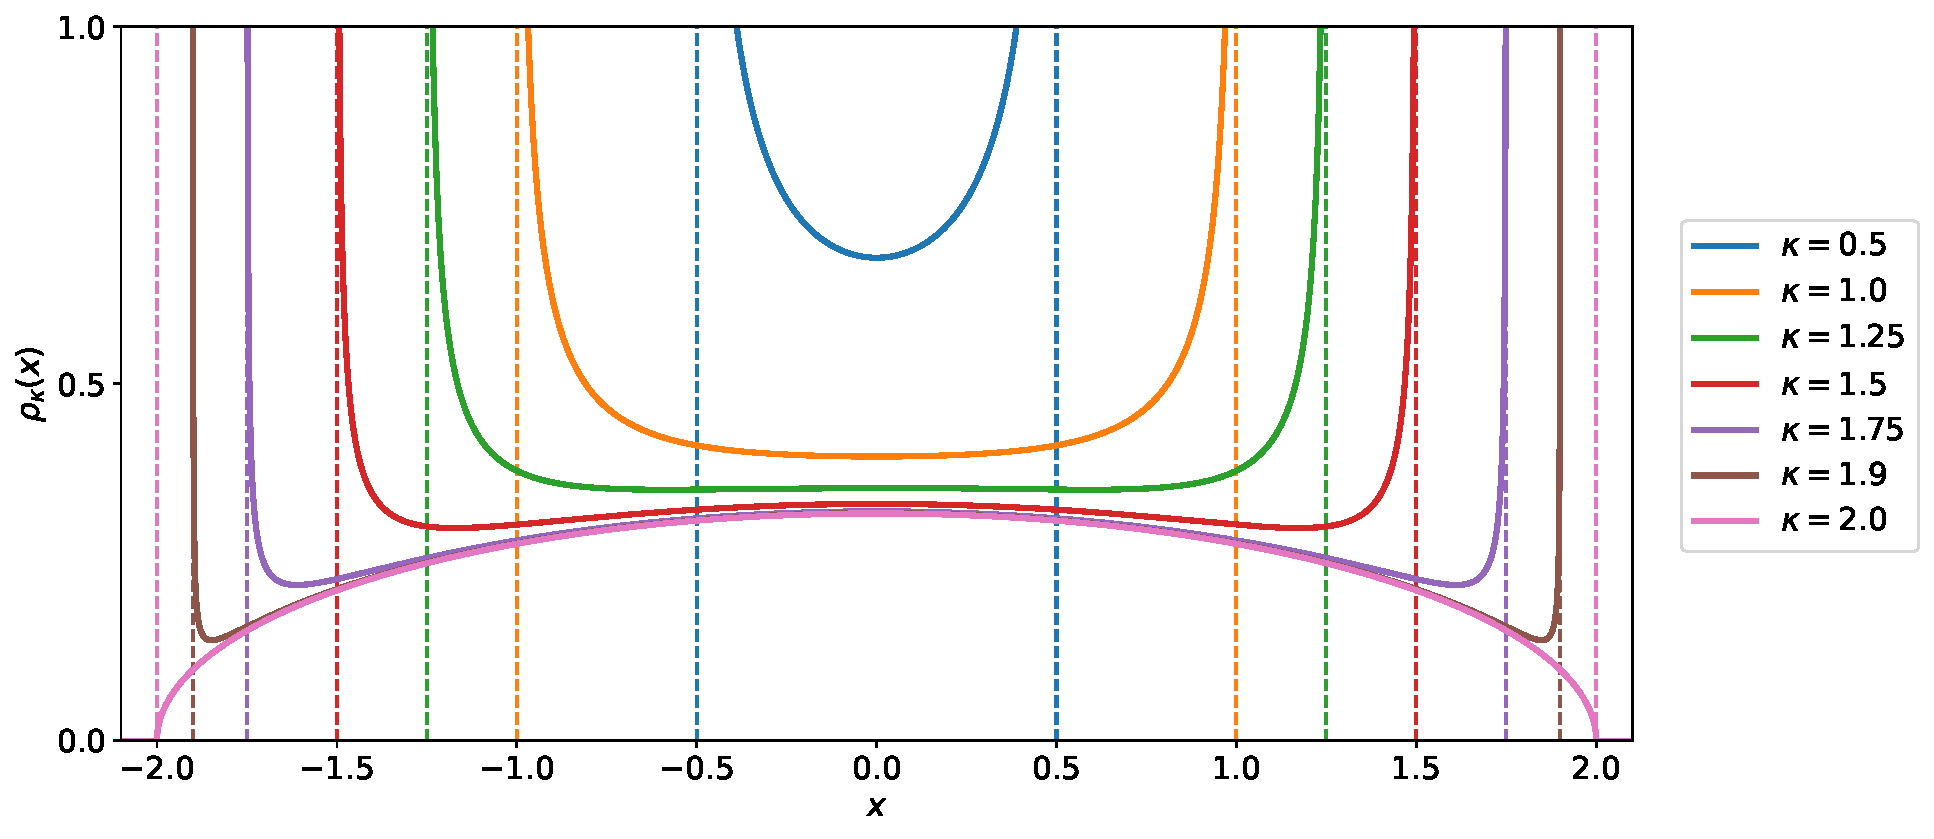
\includegraphics[width=0.8\textwidth]{figures/rho_kappa.pdf}
\caption{$\rho_\kappa(x)$ of eq.~\eqref{def:rhokappa_1} for different values of $\kappa$. For $\kappa = 2$ one recovers the semicircle law.\label{fig:rho_kappa}}
\end{figure}

\subsection{Background on large deviations}

\myskip 
Our proof leverages the main result of \cite{arous1997large}, which is a large deviation principle for the empirical eigenvalue distribution of $\GOE(d)$ matrices\footnote{
    Notice that~\cite{arous1997large} use a convention where $\GOE(d)$ matrices have off-diagonal entries with variance $1/(2d)$. We state their result adapted to our conventions.
}.
The space $\mcM_1^+(\bbR)$ of probability measures on $\bbR$ is endowed with its usual weak topology. 
It is metrizable by the Dudley metric~\citep{bogachev2007measure}:
\begin{equation}
    \label{eq:dudley}
    d(\mu, \nu) \coloneqq \left\{\left|\int f \rd \mu - \int f \rd v\right| \, : \, |f(x)| \leq 1 \textrm{ and } |f(x) - f(y)| \leq |x - y|, \, \forall (x, y) \in \bbR^2\right\}.
\end{equation}
Recall that $\Sigma(\mu) \coloneqq \int \mu(\rd x) \mu(\rd y) \log |x-y|$.
\begin{proposition}[\cite{arous1997large}]\label{prop:ldp_emeasure}
    Let $\bW \sim \GOE(d)$. 
    We denote $\mu_{\bW} \coloneqq (1/d) \sum_{i=1}^d \delta_{\lambda_i(\bW)}$ its empirical spectral distribution. 
    For $\mu \in \mcM_1^+(\bbR)$, we define: 
    \begin{equation}
        \label{eq:def_I}
        I(\mu) \coloneqq -\frac{1}{2} \Sigma(\mu) + \frac{1}{4} \int \mu(\rd x) \, x^2 - \frac{3}{8}.
    \end{equation}
    Then: 
    \begin{itemize}
        \item[$(i)$] $I : \mcM_1^+(\bbR) \to [0, \infty]$ is a strictly convex function and a good rate function, i.e.\  
        $\{I_1 \leq M\}$ is a compact subset of $\mcM_1^+(\bbR)$ for any $M > 0$.
        \item[$(ii)$]
        The law of $\mu_\bW$ satisfies a large deviation principle, in the scale $d^2$, with rate function $I$, that is for any 
        open (respectively closed) subset $O \subseteq \mcM_1^+(\bbR)$ (respectively $F \subseteq \mcM_1^+(\bbR)$): 
        \begin{equation*}
            \begin{dcases}
                \liminf_{d\to\infty} \frac{1}{d^2} \log \bbP[\mu_\bW \in O] \geq - \inf_{\mu \in O} I(\mu), \\
                \limsup_{d\to\infty} \frac{1}{d^2} \log \bbP[\mu_\bW \in F] \leq - \inf_{\mu \in F} I(\mu).
            \end{dcases}
        \end{equation*}
    \end{itemize}
\end{proposition}

\myskip
\textbf{More general large deviations results --}
\cite{arous1997large} also prove large deviations results for the empirical measure of $\bW$ sampled under more general distributions, with density 
proportional to $\exp\{-\Tr[V(\bW)]\}$, for a continuous potential $V$ growing fast enough at infinity, see also Section~2.6 of \cite{anderson2010introduction}. 
One could approach Proposition~\ref{prop:ldp_Wop} by noticing that
the law of $\bW \sim \GOE(d)$ constrained to $\|\bW\|_\op \leq \kappa$ can be written in this form, with a discontinuous potential
$V(x) = x^2 + \indi\{|x| > \kappa\} \times \infty$.
However, we will see that the large deviations of the empirical measure is only used to prove the upper bound in Proposition~\ref{prop:ldp_Wop}, 
and the particular form of the operator norm constraint allows us to rely solely on Proposition~\ref{prop:ldp_emeasure}, rather than 
adapting the general results of \cite{arous1997large,anderson2010introduction} to this discontinuous potential. 

\subsection{Large deviation upper bound for the operator norm}\label{subsec:ldp_Wop_ub}

We prove here the upper bound for $(1/d^2) \log \bbP[\|\bW\|_\op \leq \kappa]$ in Proposition~\ref{prop:ldp_Wop}.

\myskip
Let $Q \coloneqq \{\mu \in \mcM_1^+(\bbR) \, : \, \mu([-\kappa, \kappa]) = 1\}$. 
By the Portmanteau theorem, $Q$ is sequentially closed under weak convergence, and thus closed since the weak topology on $\mcM_1^+(\bbR)$ is metrizable.
We apply Proposition~\ref{prop:ldp_Wop} to get:
\begin{align}
    \label{eq:ub_ldp_Wop}
    \nonumber
     \limsup_{d \to \infty} \frac{1}{d^2} \log \bbP[\|\bW\|_\op \leq \kappa] &=  \limsup_{d \to \infty} \frac{1}{d^2} \log \bbP[\mu_\bW \in Q] , \\ 
    \nonumber
     &\leq - \inf_{\mu \in Q} I(\mu), \\ 
     &= - \inf_{\mu \in \mcM_1^+([-\kappa,\kappa])} I(\mu).
\end{align}
The last equality follows since $I(\mu_{|[-\kappa,\kappa]}) = I(\mu)$ for all $\mu \in Q$, see eq.~\eqref{eq:def_I}.
In order to characterize the minimizer of $I(\mu)$ for $\mu \in \mcM_1^+([-\kappa,\kappa])$, we
rely on classical results of logarithmic potential theory, such as Theorem~1.3 of Chapter~I of \cite{saff2013logarithmic}, see also \cite{mhaskar1985does} and Theorem~2.4 of \cite{arous1997large}.
In our context, the ``admissible weight function'' of~\cite{saff2013logarithmic} reads
\begin{equation*}
    w(x) = \exp\{-x^2/4\} \indi\{|x| \leq \kappa\}.
\end{equation*}
Adapting the results of the aforementioned literature to our notations, we obtain the following theorem.
\begin{theorem}[\cite{saff2013logarithmic}]
    \label{thm:properties_inf_I}
    ~\\
    Let $\kappa > 0$ and
    $E_\kappa \coloneqq \inf_{\mu \in \mcM_1^+([-\kappa,\kappa])} I(\mu)$. Then
    \begin{itemize}
        \item[$(i)$] $E_\kappa < \infty$.
        \item[$(ii)$] There exists a unique $\mu_\kappa^\star \in \mcM_1^+([-\kappa,\kappa])$ such that $I(\mu_\kappa^\star) = E_\kappa$.
        \item[$(iii)$] $\mu_\kappa^\star$ is the unique measure in $\mcM_1^+([-\kappa,\kappa])$ such that for $\mu_\kappa^\star$-almost all $x$: 
        \begin{equation*}
            \int \mu_\kappa^\star(\rd y) \, \log |x - y| = \frac{x^2}{4} + \frac{1}{4} \int \mu_\kappa^\star(\rd y) \, y^2 - \frac{3}{4} - 2 E_\kappa.
        \end{equation*}
    \end{itemize} 
\end{theorem}
\noindent
One can further show that this theorem allows to prove that a candidate measure is the optimal one without computing $E_\kappa$.
\begin{lemma}\label{lemma:log_pot_mukappa}
    For $\kappa \in (0,2]$, assume that $\mu \in \mcM_1^+([-\kappa,\kappa])$ and $C \in \bbR$ are such that for all $x \in (-\kappa,\kappa)$:
    \begin{equation}\label{eq:log_pot_mukappa_hyp}
        \int \mu(\rd y) \, \log |x - y| = \frac{x^2}{4} + C.
    \end{equation}
    Then $\mu = \mu_\kappa^\star$.
\end{lemma}
\noindent
Note that Lemma~\ref{lemma:log_pot_mukappa} can also be seen as a consequence of Theorem~3.3 of Chapter~I of \cite{saff2013logarithmic}. 
We give here a short proof for the sake of completeness.
\begin{proof}[Proof of Lemma~\ref{lemma:log_pot_mukappa} --]
    For any $\sigma, \nu$ real signed measures, we have (recall eq.~\eqref{eq:def_I}) 
    \begin{equation*}
        I(\sigma + \nu) - I(\sigma) = -\frac{1}{2} \Sigma(\nu) + \int \nu(\rd x) \left[\frac{x^2}{4} - \int \sigma(\rd y) \log |x - y|\right]. 
    \end{equation*}
    Applying this formula to $\sigma = \mu$ and $\nu = \mu_\kappa^\star - \mu$, we reach:
    \begin{align*}
        I(\mu_\kappa^\star) - I(\mu) &= -\frac{1}{2} \Sigma(\mu_\kappa^\star - \mu) + \int (\mu_\kappa^\star - \mu)(\rd x) \left[\frac{x^2}{4} - \int \mu(\rd y) \log |x - y|\right], \\ 
         &\aeq -\frac{1}{2} \Sigma(\mu_\kappa^\star - \mu), \\ 
         &\bgeq 0.
    \end{align*}
    We used eq.~\eqref{eq:log_pot_mukappa_hyp} in $(\rm a)$ and the fact that $\mu_\kappa^\star$ has no atom since $I(\mu_\kappa^\star) < \infty$~\citep{arous1997large}, so we can restrict the integral 
    to $x \in (-\kappa,\kappa)$.
    In $(\rm b)$ we used the following classical property of the non-commutative entropy $\Sigma(\mu)$, 
    which can be found e.g.\ as Proposition~II.2.2 in \cite{faraut2014logarithmic}.
    \begin{lemma}\label{lemma:nonc_entropy_pos}
        Let $\mu$ be a signed measure on $\bbR$ with compact support, and such that $\int_\bbR \mu(\rd x) = 0$. 
        Let $\hat{\mu}(t) \coloneqq \int \mu(\rd x) \, e^{i t x}$ be the Fourier transform of $\mu$.
        Then 
        \begin{equation*}
            \Sigma(\mu) \coloneqq \int \mu(\rd x) \mu(\rd y) \log |x - y| = - \int_0^\infty \frac{|\hat{\mu}(t)|^2}{t} \rd t.
        \end{equation*}
        In particular, $\Sigma(\mu) \leq 0$.
    \end{lemma}
    \noindent
    This shows that $I(\mu) \leq I(\mu_\kappa^\star) = \inf_{\mu \in \mcM_1^+([-\kappa,\kappa])} I(\mu)$. By $(ii)$ of Theorem~\ref{thm:properties_inf_I}, $\mu = \mu_\kappa^\star$.
\end{proof}
\noindent
Thanks to Lemma~\ref{lemma:log_pot_mukappa}, we can give an exact formula for $\mu_\kappa^\star$ by exhibiting a candidate measure satisfying eq.~\eqref{eq:log_pot_mukappa_hyp}, which in turns implies an exact formula for $E_\kappa$.
\begin{proposition}
    \label{prop:mukappa_value}
    Let $\kappa \in (0,2]$.
    Recall that $E_\kappa = \inf_{\mu \in \mcM_1^+([-\kappa,\kappa])} I(\mu)$ is reached in a unique measure $\mu_\kappa^\star$.
    Let $\mu_\kappa(\rd x) \coloneqq \rho_\kappa(x) \rd x$ be given, for $x \in (-\kappa,\kappa)$, by:
    \begin{equation}\label{eq:def_rhokappa}
        \rho_\kappa(x) \coloneqq \frac{4+\kappa^2-2x^2}{4 \pi \sqrt{\kappa^2 - x^2}}. 
    \end{equation}
    Then $\mu_\kappa = \mu_\kappa^\star$, and 
    \begin{equation*}
        E_\kappa = I(\mu_\kappa^\star) = - \frac{\kappa^4}{128} + \frac{\kappa^2}{8} - \frac{1}{2} \log \frac{\kappa}{2} - \frac{3}{8}.
    \end{equation*}
\end{proposition}
\noindent
Combining Proposition~\ref{prop:mukappa_value} with eq.~\eqref{eq:ub_ldp_Wop}, we obtain the upper bound, 
for $\kappa \in (0,2]$:
\begin{equation}
        \limsup_{d \to \infty} \frac{1}{d^2} \log \bbP[\|\bW\|_\op \leq \kappa] 
        \leq \frac{\kappa^4}{128} - \frac{\kappa^2}{8} + \frac{1}{2} \log \frac{\kappa}{2} + \frac{3}{8}.
\end{equation}
It therefore just remains to prove Proposition~\ref{prop:mukappa_value}.
\begin{proof}[Proof of Proposition~\ref{prop:mukappa_value}] 
    By Lemma~\ref{lemma:log_pot_mukappa}, to show that $\mu_\kappa = \mu_\kappa^\star$ it is enough to show that eq.~\eqref{eq:log_pot_mukappa_hyp} 
    holds for $\mu_\kappa$. 
    Since $U(x) \coloneqq \int \mu_\kappa(\rd y) \log |x-y|$ satisfies (in the sense of distributions)
    \begin{equation*}
        U'(x) = \textrm{P.V.} \int \frac{\rho_\kappa(y)}{x-y} \rd y,
    \end{equation*}
    it is enough to check for any $x \in (-\kappa,\kappa)$:
    \begin{equation}\label{eq:to_show_rhokappa}
        \textrm{P.V.}\int_{-r}^r \frac{\rho_\kappa(y)}{x-y} \rd y = \frac{x}{2}, 
    \end{equation}
    where $\textrm{P.V.}$ refers to the principal value. 
    Notice that
    \begin{equation*}
        \textrm{P.V.}\int_{-r}^r \frac{\rho_\kappa(y)}{x-y} \rd y = \lim_{\eps \downarrow 0} \Re\left\{\int_{-r}^r \frac{\rho_\kappa(y)}{x+i\eps-y} \rd y\right\}.
    \end{equation*}
    We compute $G_\kappa(z) \coloneqq \int_{-r}^r \rho_\kappa(y)/(z-y) \rd y$ for all $z$ such that $\Im(z) > 0$.
    Changing variables to $y = \kappa \cos \theta$, and then to $\zeta = e^{i \theta}$, we have:
    \begin{align*}
        G_\kappa(z) &= \frac{1}{4\pi} \int_0^\pi \frac{4+\kappa^2 -2 \kappa^2 \cos^2 \theta}{z - \kappa \cos \theta} \, \rd \theta, \\ 
        &= \frac{1}{8\pi} \int_{-\pi}^\pi \frac{4+\kappa^2 -2 \kappa^2 \cos^2 \theta}{z - \kappa \cos \theta} \, \rd \theta, \\
        &= \frac{1}{8 i\pi} \oint_{|\zeta| = 1} \frac{\kappa^2 \zeta^4 - 8 \zeta^2 + \kappa^2}{\zeta^2(\kappa\zeta^2 -2 \zeta z + \kappa)} \rd \zeta.
    \end{align*}
    The denominator has three poles: $\{0, \zeta_-, \zeta_+\}$, where $\zeta_{\pm} \coloneqq (z \pm \sqrt{z^2-\kappa^2})/\kappa$ (we choose the branch of the square root such that $\Im[\sqrt{w}] \geq 0$ for all $w \in \bbC$).
    Since $\Im(z) > 0$, it is easy to show that $|\zeta_-| < 1 < |\zeta_+|$.
    We then apply the residue theorem and find:
    \begin{equation}\label{G_rhokappa}
        G_\kappa(z) = \frac{z}{2} + \frac{4+\kappa^2-2z^2}{4\sqrt{z^2-\kappa^2}}.
    \end{equation}
    Taking $\lim_{\eps \to 0} \Re[G_\kappa(x+i \eps)]$ for $|x| < \kappa$ yields eq.~\eqref{eq:to_show_rhokappa}, and thus $\mu_\kappa = \mu_\kappa^\star$. 
    It remains to compute $E_\kappa = I(\mu_\kappa^\star)$.
    One can use the same arguments as above (based on the residue theorem) to show 
    \begin{equation}
        \label{eq:int_mukappa_x2}
        \int \mu_\kappa^\star(\rd x) \, x^2 = \frac{\kappa^2(8-\kappa^2)}{16}. 
    \end{equation}
    By $(iii)$ of Theorem~\ref{thm:properties_inf_I} and Lemma~\ref{lemma:log_pot_mukappa},
    we then have for all $x \in (-\kappa,\kappa)$:
    \begin{equation}
        \label{eq:Ekappa_1}
        E_\kappa = \frac{\kappa^2(8-\kappa^2)}{128} - \frac{3}{8} + \frac{x^2}{8} - \frac{1}{2} \int_{-\kappa}^\kappa \rho_\kappa(y) \, \log |x-y| \, \rd y.  
    \end{equation}
    Notice that eq.~\eqref{G_rhokappa} is valid for all $z$ with $\Im(z) > 0$. In particular, we reach from it, that for all $x \geq 0$:
    \begin{equation*}
        \textrm{P.V.}\int_{-r}^r \frac{\rho_\kappa(y)}{x-y} \rd y =
        \begin{dcases}
            \frac{x}{2} & \textrm{ if } x < \kappa, \\ 
            \frac{x}{2} + \frac{4+\kappa^2-2x^2}{4\sqrt{x^2-\kappa^2}} & \textrm{ if } x > \kappa.
        \end{dcases}
    \end{equation*}
    Since this is an integrable function, we have
    \begin{equation*}
        \int_{-\kappa}^\kappa \rho_\kappa(y) \, \log |x-y| \, \rd y =
        \begin{dcases}
            \frac{x^2}{4} + C & \textrm{ if } x \leq \kappa, \\ 
            \frac{x^2}{4} + C - \frac{x\sqrt{x^2-\kappa^2}}{4} - \log\left(\frac{x-\sqrt{x^2-\kappa^2}}{\kappa}\right) & \textrm{ if } x > \kappa.
        \end{dcases}
    \end{equation*}
    Using that $\int_{-\kappa}^\kappa \rho_\kappa(y) \log |x-y| \rd y - \log x \to 0$ as $x \to \infty$ yields $C = \log(\kappa/2) - \kappa^2/8$.
    Eq.~\eqref{eq:Ekappa_1} becomes:
    \begin{align*}
        E_\kappa = I(\mu_\kappa^\star) &= \frac{\kappa^2(8-\kappa^2)}{128} - \frac{3}{8}  - \frac{1}{2} \left[\log \frac{\kappa}{2} - \frac{\kappa^2}{8}\right], \\ 
        &= - \frac{\kappa^4}{128} + \frac{\kappa^2}{8} - \frac{1}{2} \log \frac{\kappa}{2} - \frac{3}{8},
    \end{align*}
    which ends the proof.
\end{proof}
\myskip
\textbf{Remark: predicting the form of $\rho_\kappa$ --} In order to predict the density $\rho_\kappa$ given by eq.~\eqref{eq:def_rhokappa}, 
we used an argument based on a heuristic application of Tricomi's theorem~\citep{tricomi1985integral}, which states that if eq.~\eqref{eq:to_show_rhokappa} is satisfied 
and $\rho_\kappa$ is supported on $[-\kappa,\kappa]$, then 
\begin{equation}\label{eq:tricomi}
    \rho_\kappa(x) = \frac{1}{\pi \sqrt{\kappa^2-x^2}}\left[C - \frac{1}{\pi} \textrm{P.V.} \int_{-\kappa}^\kappa \frac{\sqrt{\kappa^2-y^2}}{x-y} \times \left(\frac{y}{2}\right) \rd y\right],
\end{equation}
for some constant $C$ chosen to ensure $\int_{-\kappa}^\kappa \rho_\kappa(x) \rd x = 1$.
A careful evaluation of eq.~\eqref{eq:tricomi} based on the residue theorem yields eq.~\eqref{eq:def_rhokappa}.

\subsection{Large deviation lower bound for the operator norm}

We focus now on the lower bound for $(1/d^2) \log \bbP[\|\bW\|_\op \leq \kappa]$ in Proposition~\ref{prop:ldp_Wop}.

\myskip
Unfortunately the large deviation statement of Proposition~\ref{prop:ldp_emeasure} is not enough to obtain the corresponding lower bound to eq.~\eqref{eq:ub_ldp_Wop}, 
because the set of probability measures supported in $[-\kappa,\kappa]$ has empty interior under the weak topology\footnote{For any $\mu \in \mcM_1^+(\bbR)$, there is a sequence $\mu_n$ weakly converging to $\mu$ while $ \supp(\mu_n) \nsubseteq [-\kappa,\kappa]$.}. 
Instead, we come back to the joint law of the eigenvalues of a $\GOE(d)$ matrix, and 
restrict the integration domain to a small neighborhood of the quantiles of $\mu_\kappa^\star$.
This strategy is similar to the one used in the proof of the large deviation lower bound in \cite{arous1997large}.

\myskip 
The joint law of the eigenvalues $(\lambda_1, \cdots, \lambda_d)$ of $\bW$ is well-known thanks to the rotation invariance of the law of $\bW$. 
We have (see e.g.\ Theorem~2.5.2 of \cite{anderson2010introduction}):
\begin{align}\label{eq:joint_law_evalues}
    \bbP[\|\bW\|_\op \leq \kappa] &= \frac{\int_{[-\kappa,\kappa]^d} \prod_{i < j} |\lambda_i - \lambda_j| e^{-\frac{d}{4} \sum_{i=1}^d \lambda_i^2} \prod_{i=1}^d \rd \lambda_i}{\int_{\bbR^d} \prod_{i < j} |\lambda_i - \lambda_j| e^{-\frac{d}{4} \sum_{i=1}^d \lambda_i^2} \prod_{i=1}^d \rd \lambda_i}.
\end{align}
The denominator (or partition function) can be computed from Selberg's integrals~\citep{mehta2014random}.
Its limit is given by
\begin{align}\label{eq:part_function_selberg}
    \lim_{d \to \infty} \frac{1}{d^2} \log \int_{\bbR^d} \prod_{i < j} |\lambda_i - \lambda_j| e^{-\frac{d}{4} \sum_{i=1}^d \lambda_i^2} \prod_{i=1}^d \rd \lambda_i 
    &= - \frac{3}{8}.
\end{align}
Let $\delta \in (0,\kappa)$, and recall the definition of $\rho_\kappa$ in eq.~\eqref{eq:def_rhokappa}.
In what follows, we let $\nu_\delta \coloneqq \rho_{\kappa - \delta}$.
We define the quantiles of $\nu_\delta$ as 
\begin{equation*}
    -(\kappa-\delta) = x_0^{(d)} < x_1^{(d)} < \cdots < x_d^{(d)} < x_{d+1}^{(d)} = \kappa - \delta, 
\end{equation*}
with, for all $i \in \{0, \cdots, d\}$:
\begin{equation*}
    \int_{x_i^{(d)}}^{x_{i+1}^{(d)}} \nu_\delta(u) \, \rd u = \frac{1}{d+1}. 
\end{equation*}
We will drop the subscript and write $x_i$ for $x_i^{(d)}$ to lighten notations.

\myskip
Clearly, the empirical measure $(1/d)\sum_{i=1}^d \delta_{x_i}$ weakly converges to $\nu_\delta$ as $d \to \infty$.
Notice that $\{(\lambda_i)_{i=1}^d \, : \, |\lambda_i - x_i| \leq \delta, \, \, \forall i \in [1,d]\} \subseteq [-\kappa,\kappa]^d$, 
so that from eqs.~\eqref{eq:joint_law_evalues} and \eqref{eq:part_function_selberg}:
\begin{align}
    \label{eq:lb_Wop_1}
   &e^{-\frac{3d^2}{8} + \smallO(d^2)} \bbP[\|\bW\|_\op \leq \kappa] \\ 
    \nonumber
   &\geq \int_{[-\delta,\delta]^d} \prod_{i < j} |u_i - u_j + x_i - x_j| e^{-\frac{d}{4} \sum_{i=1}^d (u_i + x_i)^2} \prod_{i=1}^d \rd u_i,\\ 
    \nonumber
   &\ageq \int_{[-\delta,\delta]^d \cap \Delta_d} \prod_{i < j} (u_j - u_i + x_j - x_i) e^{-\frac{d}{4} \sum_{i=1}^d (u_i + x_i)^2} \prod_{i=1}^d \rd u_i, \\
    \nonumber
   &\bgeq \int_{[-\delta,\delta]^d \cap \Delta_d} \prod_{i + 1< j} (x_j - x_i) \prod_{i=1}^{d-1} [x_{i+1} - x_{i}]^{1/2} [u_{i+1} - u_i]^{1/2} e^{-\frac{d}{4} \sum_{i=1}^d (\delta + |x_i|)^2} \prod_{i=1}^d \rd u_i,
\end{align}
where we defined in $(\rm a)$ the set $\Delta_d \coloneqq \{u_1 < \cdots < u_d\}$, and used 
in $(\rm b)$ that $u_i \leq u_j$ and $x_i \leq x_j$, as well as the inequality $A+B \geq \sqrt{AB}$ for $A, B \geq 0$.
The integral on the variables $u_i$ can be lower-bounded as follows:
\begin{align}\label{eq:volume_u}
    \nonumber
    \int_{[-\delta,\delta]^d \cap \Delta_d} \prod_{i=1}^{d-1} \sqrt{u_{i+1} - u_i} \prod_{i=1}^d \rd u_i 
    &= \delta^{(3d-1)/2} \int_{[-1,1]^d \cap \Delta_d} \prod_{i=1}^{d-1} \sqrt{u_{i+1} - u_i} \prod_{i=1}^d \rd u_i , \\ 
    \nonumber
    &\geq \delta^{(3d-1)/2} \prod_{i=1}^{d} \int_{-1 + \frac{2(i-1)}{d}}^{-1 + \frac{2i-1}{d}} \rd u_i \, \left(\prod_{i=1}^{d-1} \sqrt{u_{i+1} - u_i}\right) , \\ 
    &\geq \left(\frac{\delta}{d}\right)^{(3d-1)/2}.
\end{align}
Combining eqs.~\eqref{eq:lb_Wop_1} and \eqref{eq:volume_u}: 
\begin{align*}
    \liminf_{d \to \infty} \frac{1}{d^2} \log \bbP[\|\bW\|_\op \leq \kappa]  
    &\geq \frac{3}{8} - \frac{\delta^2}{4}
    + \liminf_{d \to \infty} \left[-\frac{\delta}{2d} \sum_{i=1}^d |x_i| -\frac{1}{4d} \sum_{i=1}^d x_i^2\right. \\ 
    &\left.+ \frac{1}{2d^2} \sum_{i=1}^{d-1} \log (x_{i+1} - x_i) + \frac{1}{d^2} \sum_{i,j=1}^d \log(x_j - x_i) \indi\{j > i+1\}
    \right].
\end{align*}
By the weak convergence described above, and since $\sum_{i=1}^d x_i^2 = \sum_{i=1}^d x_i^2 \indi\{|x_i| \leq \kappa\}$, we get by the Portmanteau theorem:
\begin{align}\label{eq:lb_Wop_2}
    \liminf_{d \to \infty} \frac{1}{d^2} \log \bbP[\|\bW\|_\op \leq \kappa]  
    &\geq \frac{3}{8} - \frac{\delta^2}{4} - \frac{\delta}{2} \int |x| \nu_\delta(\rd x) - \frac{1}{4} \int x^2 \nu_\delta(\rd x) \\
    \nonumber
    &\hspace{-9pt}+ \liminf_{d \to \infty}\left[\frac{1}{2d^2} \sum_{i=1}^{d-1} \log (x_{i+1} - x_i) + \frac{1}{d^2} \sum_{i,j=1}^d \log(x_j - x_i) \indi\{j > i+1\}
    \right].
\end{align}
Finally, notice that 
\begin{align*}
    \Sigma(\nu_\delta) &= 2 \sum_{0 \leq i,j \leq d} \int_{x_i}^{x_{i+1}} \nu_\delta(\rd x) \int_{x_j}^{x_{j+1}} \nu_\delta(\rd y) \, \log (y-x) \, \indi\{x < y\}, \\ 
    &\leq \sum_{i=0}^d \int_{x_i}^{x_{i+1}} \nu_\delta(\rd x) \int_{x_i}^{x_{i+1}} \nu_\delta(\rd y) \, \log |y-x| + 2 \sum_{0 \leq i < j \leq d} \frac{\log(x_{j+1} - x_i)}{(d+1)^2}, \\
    &\leq \frac{1}{(d+1)^2} \left[\sum_{i=0}^d \log(x_{i+1}-x_i) + 2 \sum_{0 \leq i < j \leq d} \log(x_{j+1} - x_i)\right], \\ 
    &\aleq \frac{1}{(d+1)^2} \left[\sum_{i=1}^{d-1} \log(x_{i+1}-x_i) + 2 \sum_{i,j=1}^d \log(x_j - x_i) \indi\{j > i+1\} \right] + \frac{2d+1}{(d+1)^2} \log 2 \kappa.
\end{align*}
We used in $(\rm a)$ that $|x_i - x_j| \leq 2 (\kappa-\delta) \leq 2\kappa$ for all $i,j$.
Using this in eq.~\eqref{eq:lb_Wop_2} gives:
\begin{align*}
    \liminf_{d \to \infty} \frac{1}{d^2} \log \bbP[\|\bW\|_\op \leq \kappa]  
    &\geq \frac{3}{8} - \frac{\delta^2}{4} - \frac{\delta}{2} \int |x| \nu_\delta(\rd x) - \frac{1}{4} \int x^2 \nu_\delta(\rd x) + \frac{1}{2} \Sigma(\nu_\delta), \\
    &\geq - \frac{\delta}{2} \int |x| \nu_\delta(\rd x)  - \frac{\delta^2}{4} - I(\nu_\delta).
\end{align*}
Recall that $\nu_\delta = \rho_{\kappa - \delta}$, so that taking the limit $\delta \to 0$, we get:
\begin{align*}
    \liminf_{d \to \infty} \frac{1}{d^2} \log\bbP[\|\bW\|_\op \leq \kappa] 
    &\geq - I(\rho_\kappa),
\end{align*}
Proposition~\ref{prop:mukappa_value} gives the value of $I(\rho_\kappa)$, which implies the lower bound
\begin{align}\label{eq:lb_ldp_Wop}
        \liminf_{d \to \infty} \frac{1}{d^2} \log \bbP[\|\bW\|_\op \leq \kappa] 
        \geq \frac{\kappa^4}{128} - \frac{\kappa^2}{8} + \frac{1}{2} \log \frac{\kappa}{2} + \frac{3}{8}.
\end{align}
Combining eqs.~\eqref{eq:ub_ldp_Wop} and \eqref{eq:lb_ldp_Wop} ends the proof of Proposition~\ref{prop:ldp_Wop}.
$\qed$

\subsection{Limiting spectral distribution of a norm-constrained Gaussian matrix}\label{subsec:proof_lsd_constrained_GOE}

We prove here Theorem~\ref{thm:lsd_constrained_GOE}.
A large deviations upper bound for the law of $\mu_\bW$ can be obtained by combining Proposition~\ref{prop:ldp_emeasure} 
and Proposition~\ref{prop:ldp_Wop}, as we state in the following corollary.
\begin{corollary}
    \label{cor:ldp_ub}
    Let $\kappa \in (0,2]$ and $\bW \sim \bbP_\kappa$. 
    We denote $\mu_{\bW} \coloneqq (1/d) \sum_{i=1}^d \delta_{\lambda_i(\bW)}$ its empirical spectral distribution. 
    Recall the definition of $I(\mu)$ in eq.~\eqref{eq:def_I}, and of $\mu_\kappa^\star(\rd x) =\rho_\kappa(x) \rd x$ in eq.~\eqref{eq:def_rhokappa}.
    Then the law of $\mu_\bW$ satisfies a large deviation upper bound, in the scale $d^2$, with rate function 
    $J_\kappa(\mu) \coloneqq I(\mu) - I(\mu_\kappa^\star)$,
    that is for any closed subset $F \subseteq \mcM_1^+([-\kappa,\kappa])$: 
    \begin{align*}
            \limsup_{d\to\infty} \frac{1}{d^2} \log \bbP_\kappa[\mu_\bW \in F] \leq - \inf_{\mu \in F} J_\kappa(\mu).
    \end{align*}
\end{corollary}
\begin{proof}[Proof of Corollary~\ref{cor:ldp_ub}]
    Because $\mu_\bW \in F \Rightarrow \|\bW\|_\op \leq \kappa$, we have 
    \begin{align*}
       \bbP_\kappa[\mu_\bW \in F] &= \bbP_{\bW \sim \GOE(d)}[\mu_\bW \in F \, | \, \|\bW\|_\op \leq \kappa], \\
       &= \frac{\bbP_{\bW \sim \GOE(d)}[\mu_\bW \in F]}{\bbP_{\bW \sim \GOE(d)}[\|\bW\|_\op \leq \kappa]}.
    \end{align*}
    Since $F$ is closed in $\mcM_1^+([-\kappa,\kappa])$ under the weak topology, it is closed as well in $\mcM_1^+(\bbR)$.
    Thus:
    \begin{align*}
       \limsup_{d \to \infty} \frac{1}{d^2} \log \bbP_\kappa[\mu_\bW \in F] &\aeq \limsup_{d \to \infty} \frac{1}{d^2} \log \bbP_{\bW \sim \GOE(d)}[\mu_\bW \in F] + I(\mu_\kappa^\star), \\ 
       &\bleq - \inf_{\mu \in F} J_\kappa(\mu),
    \end{align*}
    using Proposition~\ref{prop:ldp_Wop} in $(\rm a)$, and Proposition~\ref{prop:ldp_emeasure} in $(\rm b)$.
\end{proof}
\noindent
While we surely anticipate that one can obtain a corresponding large deviation lower bound for $\mu_\bW$ (and thus a full large deviation principle), 
Corollary~\ref{cor:ldp_ub} is enough to imply Theorem~\ref{thm:lsd_constrained_GOE}.
Indeed, for any $\delta > 0$, if $B(\mu_\kappa^\star,\delta) \subseteq \mcM_1^+([-\kappa,\kappa])$ is the open ball of radius $\delta$ centered in $\mu_\kappa^\star$ for the distance of eq.~\eqref{eq:dudley}, 
then 
\begin{align*}
    \limsup_{d \to \infty} \frac{1}{d^2} \log \bbP_\kappa[\mu_\bW \notin B(\mu_\kappa^\star, \delta)] \leq - \inf_{\mu \in B(\mu_\kappa^\star, \delta)^c} [J_\kappa(\mu)].
\end{align*}
Since $J_\kappa$ is a good rate function (see Proposition~\ref{prop:ldp_emeasure}) and has a unique minimizer (cf.\ $(ii)$ of Theorem~\ref{thm:properties_inf_I}), 
$\inf_{\mu \in B(\mu_\kappa^\star, \delta)^c} [J_\kappa(\mu)] > 0$. Therefore, by the Borel-Cantelli lemma,
\begin{align*}
    \bbP[\limsup_{d \to \infty} d(\mu_\bW, \mu_\kappa^\star) \leq \delta] = 1,
\end{align*}
which ends the proof by taking the limit $\delta \to 0$.
$\qed$
